% Compilem amb pdfLaTeX, dues passades, des d'aquesta carpeta.
% Conservem figures_practica_2_1/ al costat d'aquest fitxer.
\documentclass[11pt,a4paper]{article}
\usepackage[utf8]{inputenc}
\usepackage[T1]{fontenc}
\usepackage{lmodern}
\usepackage[catalan]{babel}
\usepackage[margin=20mm]{geometry}
\usepackage{graphicx,booktabs,array,amsmath,xcolor}
\usepackage[font=small,labelfont=bf,skip=5pt,hypcap=false]{caption}
\usepackage[unicode,hidelinks]{hyperref}
\hypersetup{pdftitle={Pràctica 2.1: classificació d'intencions amb PyTorch},pdfauthor={}}
\definecolor{accent}{RGB}{25,55,80}
\setlength{\parindent}{0pt}
\setlength{\parskip}{5pt}
\setlength{\tabcolsep}{6pt}
\renewcommand{\arraystretch}{1.07}
\emergencystretch=2em
\raggedbottom
\newcommand{\intent}[1]{\texttt{\detokenize{#1}}}
\newcommand{\pendent}[1]{\texttt{[#1]}}
\begin{document}

{\color{accent}\LARGE\bfseries Pràctica 2.1\par}
{\Large Classificació d'intencions amb PyTorch\par}
\vspace{4pt}
\pendent{ASSIGNATURA}\par
\pendent{NOMS I COGNOMS DELS INTEGRANTS}\par
\pendent{GRUP DE PRÀCTIQUES}\hfill\pendent{DATA DE LLIURAMENT}
\vspace{5pt}\hrule\vspace{4pt}

\section{Introducció i objectius}
Hem estudiat la classificació de consultes en intencions, una tasca que permet orientar la resposta d'un sistema conversacional. Una frase pot compartir vocabulari amb una altra i demanar informació diferent; per això comparem tant representacions lèxiques agregades com models que processen patrons locals o context seqüencial.

Hem implementat tokenització, padding, codificació d'etiquetes i un model inicial. Després hem comparat vocabulari, normalització, embeddings, CNN, LSTM, GRU, bidireccionalitat, atenció, dropout i ponderació de classes. Hi afegim una parella exploratòria de self-attention amb i sense posicions. Busquem descriure efectes observats sota controls comuns, no afirmar superioritat universal ni fer una cerca exhaustiva.

\section{Conjunt de dades i preprocessament}
Hem utilitzat les dades ATIS facilitades a la pràctica, amb oracions en anglès i consultes sobre vols i serveis relacionats. Tractem cada cadena d'etiqueta, incloses les combinacions amb el signe \(+\), com una classe completa. No descomponem les etiquetes compostes en un problema multietiqueta.

\begin{center}
\captionof{table}{Particions utilitzades. Les classes es compten després del filtratge.}
\begin{tabular}{lrrr}
\toprule
Partició & Exemples originals & Exemples utilitzats & Classes presents\\
\midrule
Train & 4078 & 4078 & 22\\
Validation & 900 & 900 & 17\\
Test & 893 & 888 & 16\\
\bottomrule
\end{tabular}
\end{center}

La divisió del CSV d'entrenament conserva les primeres 4078 files per a train i les 900 finals per a validació. No és una nova partició estratificada. Excloem cinc exemples de test amb etiquetes absents de train: dos de \intent{day_name} i un de \intent{airfare+flight}, \intent{flight+airline} i \intent{flight_no+airline}. El mateix filtre no elimina cap exemple de validació. Avaluem, doncs, classes conegudes; no mesurem detecció d'intencions noves.

Hem tokenitzat per paraules, amb PAD=0, UNK=1 i paraules conegudes des de 2. El límit de vocabulari inclou els dos índexs reservats. Amb límit 500 aprenem 498 paraules i utilitzem 500 files d'embedding. UNK conserva una posició desconeguda, però no en recupera el significat. Aprenem vocabulari i longitud màxima només amb train; apliquem padding post i conservem les longituds efectives. La longitud màxima observada és 48.

La distribució és desigual: \intent{flight} conté 3023 de 4078 exemples de train (74,13\%). Quatre classes tenen una mostra i dues en tenen dues. Verifiquem 93 textos diferents compartits entre train i validació, presents en 104 files de validació, i 10 textos compartits entre train i test. Les files originals de train i validació són disjuntes, però no ho són tots els textos; no assumim independència textual.

\newpage
\section{Model inicial i metodologia experimental}
\subsection*{Arquitectura i entrenament}
El model inicial transforma cada ID en un embedding de 64 dimensions, aplica global max pooling emmascarat, una capa lineal de 64 unitats amb ReLU i una capa final de 22 logits. Excloem PAD del màxim perquè els zeros no substitueixin activacions negatives. Utilitzem \texttt{CrossEntropyLoss} amb índexs enters i sense softmax final explícit; aquesta pèrdua ja incorpora la normalització necessària~\cite{ce}.

En el model didàctic de l'exercici 4 utilitzem Adam, learning rate 0,001, batch 32, màxim 30 èpoques i patience 3. En l'execució analitzada obtenim 840/900 encerts de validació (93,33\%), best validation loss 0,3007 i aturada a l'època 23. Aquest entrenament no fixa llavor; no el confonem amb el baseline controlat de l'exercici 5 ni interpretem diferències entre reexecucions com a efectes causals.

\begin{center}
\captionof{table}{Protocol comú de l'exercici 5.}
\begin{tabular}{ll}
\toprule
Element & Configuració\\
\midrule
Optimitzador / learning rate & Adam / 0,001\\
Batch / màxim d'èpoques & 32 / 25\\
Early stopping & Patience 4; validation loss sense pesos\\
Llavor dels contrastos & 42\\
Llavor dels finalistes & 42, 123 i 2026\\
Checkpoint & Pesos de validation loss mínima, restaurats\\
Selecció de configuració & Accuracy; després macro-F1 i loss\\
\bottomrule
\end{tabular}
\end{center}

\subsection*{Controls i mètriques}
Actualitzem els pesos exclusivament amb train. Fem servir validació per aturar l'entrenament i seleccionar configuracions. En models ponderats també seleccionem checkpoints amb validation loss sense pesos, de manera que el criteri d'època continua sent comú. Acumulem la loss per exemple; en l'entrenament ponderat dividim la suma de pèrdues per la suma de pesos dels targets, no pel nombre de batches.

L'accuracy mesura la proporció d'encerts. Calculem macro-F1 sobre les 22 classes de train:
\[
  F_{1,\mathrm{macro}}=\frac{1}{22}\sum_{c=1}^{22}
  \frac{2\,TP_c}{2\,TP_c+FP_c+FN_c},
\]
amb zero quan el quocient no es pot definir~\cite{f1}. Això inclou zeros per a classes sense suport en una partició; no interpretem el seu recall com una estimació observada. Llegim sempre macro-F1 i recall juntament amb els suports, perquè l'accuracy està influïda per les classes freqüents.

Hem executat 32 entrenaments de l'exercici 5: 30 de les famílies originals i dos exploratoris. Registrem 34 configuracions; dues són equivalents en tensors i model i reutilitzen l'entrenament dins de la mateixa execució. No són dos resultats independents. Els tres finalistes inclouen les tres llavors establertes.

Hem executat el notebook complet en CPU amb quatre fils, Python 3.13.0, PyTorch \texttt{2.12.1+cpu} i NumPy 2.2.4. Hem comprovat finitud de pèrdues, dimensions, alineació d'etiquetes i restauració dels pesos. Conservem resultats, historials i pesos en memòria; el notebook recrea el procés amb \emph{Restart \& Run All}, sense checkpoints externs.

\newpage
\section{Experiments i resultats}
En els contrastos individuals mantenim la llavor 42 i canviem un factor cada vegada. Les accuracies següents són de validació i s'expressen en percentatge; els F1 es mostren entre 0 i 1.

\subsection{Preprocessament i vocabulari}
Provem 250, 500, 1000 i 2000 IDs totals per contrastar cobertura lèxica i cost. Fixem el feedforward, embedding 64, hidden 64, dropout zero i el protocol comú. Un límit petit pot augmentar UNK; un de gran pot reservar paràmetres per a paraules amb molt poc suport.

\begin{center}
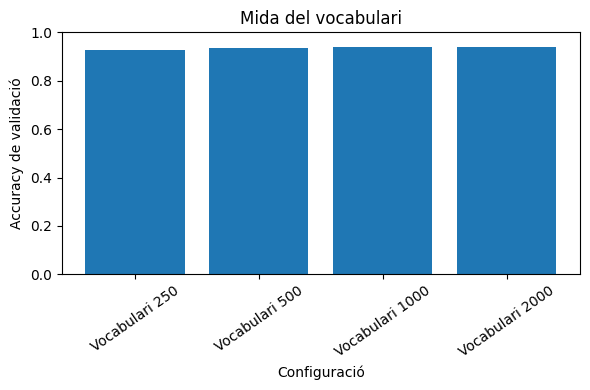
\includegraphics[width=0.72\linewidth]{figures_practica_2_1/vocabulari.png}
\captionof{figure}{Efecte del vocabulari en l'accuracy del feedforward amb embedding 64.}
\end{center}

De 250 a 1000, accuracy passa de 92,56 a 93,89\% (+1,33 punts), però macro-F1 baixa de 0,4733 a 0,4255. Amb 1000 cobrim els 830 tokens diferents de train; 2000 genera els mateixos tensors i resultat. Seleccionem 1000 per accuracy, sense afirmar una millora uniforme entre classes.

Amb vocabulari 500, lowercase activat i desactivat són equivalents: els textos de train i validació ja estan en minúscules. Stemming redueix accuracy de 93,56 a 92,89\% i macro-F1 de 0,4565 a 0,4113. Conservem stopwords com \emph{not}, \emph{from} i \emph{to}, i els números. No combinem stemming i lematització: volem aïllar una normalització i no afegir una segona intervenció.

\subsection{Dimensionalitat dels embeddings}
Comparem 32, 64 i 128 dimensions amb vocabulari 500 i hidden 64. Augmentar dimensió amplia la representació i els paràmetres; no garanteix generalització.
\begin{center}
\begin{tabular}{rrrr}
\toprule
Dimensió & Accuracy (\%) & Macro-F1 & Paràmetres\\
\midrule
32 & 90,67 & 0,3668 & 19\,542 \\
64 & 93,56 & 0,4565 & 37\,590 \\
128 & 93,67 & 0,4797 & 73\,686 \\
\bottomrule
\end{tabular}
\end{center}

De 64 a 128 afegim només un encert sobre 900, tot i gairebé duplicar paràmetres. Provem explícitament la combinació addicional vocabulari 1000 i embedding 128: obtenim 94,11\% i 0,4500 de macro-F1. La seleccionem per continuar per accuracy, encara que no supera el macro-F1 del contrast de 128 dimensions amb vocabulari 500.

\newpage
\subsection{Xarxes convolucionals}
Estudiem patrons locals amb kernels 2, 3 i 5 i 64 filtres. Fixem preprocessing comú, embedding 128 i dropout zero. Primer comparem kernels amb max pooling; després comparem pooling amb el millor kernel i afegim una segona convolució a la variant amb max. Evitem canviar alhora amplada i profunditat o fer una graella cartesiana.

\begin{center}
\captionof{table}{CNN amb representació comuna.}
\small
\begin{tabular}{lrrr}
\toprule
Configuració & Accuracy (\%) & Macro-F1 & Paràmetres\\
\midrule
Una capa, kernel 2, max & 95,56 & 0,5501 & 124\,374 \\
Una capa, kernel 3, max & 94,89 & 0,5096 & 132\,566 \\
Una capa, kernel 5, max & 92,00 & 0,4534 & 148\,950 \\
Una capa, kernel 2, average & 95,78 & 0,5668 & 124\,374 \\
Dues capes, kernel 2, max & 95,78 & 0,5676 & 132\,630 \\
\bottomrule
\end{tabular}
\end{center}

Kernel 2 supera els kernels més grans en aquesta prova. Detectar fragments locals no implica comprendre totes les relacions de la frase. A més, 33 oracions de validació tenen menys de cinc tokens: amb finestres completes de kernel 5 reben una representació zero. Considerem aquest límit una possible explicació parcial, no una causa demostrada de tots els errors.

Average pooling renormalitzat i dues convolucions obtenen la mateixa accuracy, 95,78\%. La segona guanya aproximadament 0,0007 de macro-F1 i afegeix 8256 paràmetres respecte a average d'una capa. La seleccionem pel criteri secundari; el guany petit no estableix una superioritat general de la profunditat.

\subsection{Xarxes recurrents}
Comparem LSTM i GRU per representar dependències seqüencials. LSTM manté estat ocult i de ce\lgem{}a; GRU té una estructura més compacta. Fixem hidden 128, una capa i dropout zero. Empaquetem longituds amb \texttt{pack\_padded\_sequence}; en bidireccionals concatenem els estats finals de les dues direccions.

\begin{center}
\captionof{table}{Recurrents amb les mateixes dades, embedding i entrenament.}
\small
\begin{tabular}{lrrr}
\toprule
Arquitectura & Accuracy (\%) & Macro-F1 & Paràmetres\\
\midrule
LSTM & 96,22 & 0,5455 & 241\,430 \\
BiLSTM & 97,00 & 0,6268 & 376\,342 \\
GRU & 96,67 & 0,6168 & 208\,406 \\
BiGRU & 97,00 & 0,6037 & 310\,294 \\
LSTM + atenció & 97,11 & 0,6164 & 241\,559 \\
BiLSTM + atenció & 96,78 & 0,6085 & 376\,599 \\
\bottomrule
\end{tabular}
\end{center}

Bidireccionalitat millora accuracy en LSTM i GRU, però en GRU redueix macro-F1. LSTM + atenció guanya 0,89 punts d'accuracy a LSTM i només 0,11 a BiLSTM; no supera el macro-F1 de BiLSTM. L'atenció escalar afegeix 129 paràmetres a LSTM i agrega els seus estats contextuals amb màscara, sense ser self-attention.

Atenció sobre BiLSTM empitjora les dues mètriques. Seleccionem LSTM + atenció per accuracy; amb hidden 64 baixa a 96,33\% i 0,5152 de macro-F1, davant dels 97,11\% amb hidden 128. Mantenim 128. No explorem totes les combinacions de capes, direccions i atenció: limitem cost i interaccions, i no atribuïm les diferències només a l'ordre, perquè també canvien capacitat i optimització.

\newpage
\subsection{Self-attention i embeddings posicionals}
Comparem una self-attention de quatre capçals, mitjana emmascarada i classificador, amb i sense posicions apreses. Fixem embedding 128, dropout zero, loss sense pesos, llavor 42 i el mateix protocol. Compartim la inicialització dels pesos comuns. No implementem un encoder Transformer ni usem pesos preentrenats.

Sense posicions, self-attention i mitjana no representen explícitament l'ordre. Afegir posicions permet distingir-lo. Emmascarem claus i queries PAD i gestionem files buides per evitar valors no finits.

\begin{center}
\captionof{table}{Exploració posicional amb llavor 42; temps en segons.}
\small
\begin{tabular}{lrrrr}
\toprule
Variant & Accuracy (\%) & Macro-F1 & Paràmetres & Temps\\
\midrule
Sense posicions & 93,11 & 0,4548 & 175\,382 & 8,21 \\
Amb posicions & 94,11 & 0,5065 & 181\,526 & 8,98 \\
\bottomrule
\end{tabular}
\end{center}

Amb posicions guanyem 1,00 punt d'accuracy, nou encerts de validació, i 0,0517 de macro-F1. Restaurem les èpoques 4 i 5, de loss mínima; no prenem les accuracies més altes dels logs posteriors. El resultat és compatible amb utilitat de les posicions en aquesta configuració, però afegim 6144 paràmetres i només usem una llavor. No demostrem significació ni un benefici universal. Aquesta exploració queda fora de la selecció històrica i no s'avalua a test.

\subsection{Regularització}
Seleccionem una CNN i una recurrent prometedores amb validació i comparem dropout 0, 0,2 i 0,4, mantenint la resta fixa. L'apliquem després de la representació agregada, abans del classificador; no depenem del dropout intern d'una recurrent d'una sola capa.

\begin{center}
\small
\begin{tabular}{rrrrr}
\toprule
 & \multicolumn{2}{c}{CNN seleccionada} & \multicolumn{2}{c}{LSTM + atenció}\\
Dropout & Accuracy (\%) & Macro-F1 & Accuracy (\%) & Macro-F1\\
\midrule
0 & 95,78 & 0,5676 & 97,11 & 0,6164 \\
0,2 & 95,56 & 0,5385 & 96,78 & 0,5607 \\
0,4 & 95,67 & 0,5289 & 97,11 & 0,6186 \\
\bottomrule
\end{tabular}
\end{center}
\begin{center}
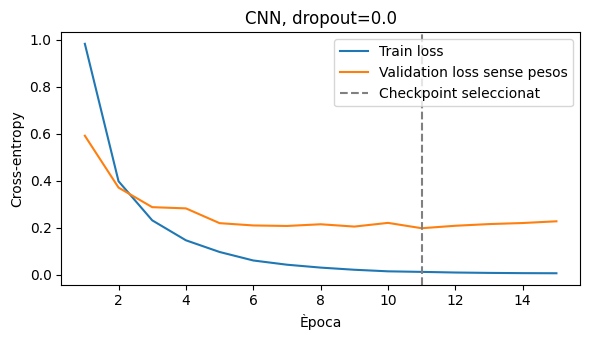
\includegraphics[width=0.70\linewidth]{figures_practica_2_1/sobreajustament_cnn.png}
\captionof{figure}{CNN sense dropout: train loss baixa mentre validation loss empitjora després del checkpoint de l'època 11.}
\end{center}

Les corbes justifiquen l'early stopping, sense demostrar que dropout elimini el sobreajustament. Conservem CNN sense dropout i LSTM + atenció amb 0,4: empata en accuracy i guanya 0,0022 de macro-F1.

\newpage
\subsection{Balanceig de classes}
La concentració en \intent{flight} pot afavorir encerts globals sense bon comportament en classes rares. Calculem pesos exclusivament amb les freqüències de train, en l'ordre de \texttt{LabelEncoder}:
\[
 w_c=\frac{N}{C\,n_c},\qquad N=4078,\quad C=22,\quad n_c>0.
\]
La fórmula iguala la contribució total nominal de cada classe quan sumem els seus pesos, però no afegeix exemples ni diversitat. La mitjana ponderada de CrossEntropyLoss es normalitza per la suma dels pesos dels targets del batch~\cite{ce}.

\begin{center}
\captionof{table}{Classe majoritària i les sis classes amb una o dues mostres de train.}
\small
\begin{tabular}{lrrr}
\toprule
Classe & Exemples & Freqüència (\%) & Pes\\
\midrule
\intent{flight} & 3\,023 & 74,13 & 0,0613 \\
\intent{restriction} & 2 & 0,05 & 92,6818 \\
\intent{airline+flight_no} & 2 & 0,05 & 92,6818 \\
\intent{aircraft+flight+flight_no} & 1 & 0,02 & 185,3636 \\
\intent{airfare+flight_time} & 1 & 0,02 & 185,3636 \\
\intent{cheapest} & 1 & 0,02 & 185,3636 \\
\intent{ground_service+ground_fare} & 1 & 0,02 & 185,3636 \\
\bottomrule
\end{tabular}
\end{center}

Una mostra d'una classe amb un únic exemple rep un pes nominal 3023 vegades superior al d'una mostra de \intent{flight}. Això pot accentuar gradients variables, memorització o sensibilitat a errors d'anotació; no hem demostrat que aquests riscos es materialitzin en cada classe.

Comparem la mateixa LSTM + atenció amb dropout 0,4, amb i sense pesos. L'accuracy es manté en 97,11\%, mentre que macro-F1 passa de 0,6186 a 0,6451. Mantenim validation loss sense pesos per seleccionar checkpoints i no barregem aquests valors amb la train loss ponderada.

\begin{center}
\captionof{table}{Canvis de recall de validació. El suport és imprescindible per interpretar-los.}
\small
\begin{tabular}{lrrr}
\toprule
Classe & Suport & Sense pesos & Amb pesos\\
\midrule
\intent{aircraft} & 13 & 0,9231 & 1,0000 \\
\intent{airport} & 6 & 0,6667 & 0,8333 \\
\intent{flight_time} & 8 & 0,8750 & 1,0000 \\
\intent{restriction} & 4 & 0,0000 & 0,2500 \\
\intent{airline} & 32 & 0,8750 & 0,9063 \\
\intent{flight+airfare} & 6 & 0,6667 & 0,8333 \\
\intent{flight} & 643 & 0,9953 & 0,9860 \\
\intent{meal} & 3 & 0,0000 & 0,0000 \\
\bottomrule
\end{tabular}
\end{center}

Cadascuna de les millores mostrades correspon a un exemple correcte addicional. En \intent{flight} passem de 640 a 634 encerts sobre 643 casos; les altres millores compensen aquesta pèrdua. En \intent{meal} no millorem. Amb quatre exemples, el recall de \intent{restriction} canvia en 0,25 per un sol cas, fet que il·lustra la fragilitat d'aquestes estimacions.

Conservem el model ponderat pel macro-F1 superior amb la mateixa accuracy, no perquè els pesos hagin eliminat el desbalanceig. Cinc classes de train no tenen suport en validació; no podem validar-hi un benefici. Tampoc una o dues mostres permeten estimar amb precisió variabilitat dins de la classe. No fem una cerca addicional de remostreig o pesos suavitzats després de veure test.

\newpage
\section{Comparació global i selecció del model}
Hem repetit un candidat de cada família original amb les llavors 42, 123 i 2026. La taula mostra mitjana i desviació mostral; en accuracy la desviació s'expressa en punts percentuals.

\begin{center}
\captionof{table}{Validació amb tres llavors (mitjana i desviació mostral); paràmetres i temps de la llavor 42.}
\small
\begin{tabular}{lrrrr}
\toprule
Finalista & Accuracy (\%) & Macro-F1 & Paràmetres & Temps (s)\\
\midrule
Feedforward & 93,74 $\pm$ 0,46 & 0,4400 $\pm$ 0,0189 & 116\,182 & 6,33 \\
CNN, dues convolucions & 96,00 $\pm$ 0,38 & 0,5617 $\pm$ 0,0230 & 132\,630 & 8,93 \\
LSTM + atenció, ponderada & 97,30 $\pm$ 0,23 & 0,6531 $\pm$ 0,0209 & 241\,559 & 26,87 \\
\bottomrule
\end{tabular}
\end{center}

Seleccionem la família recurrent per accuracy mitjana i utilitzem macro-F1 com a segon criteri. També lidera macro-F1 entre aquests tres finalistes. Això no equival a haver refet tota la cerca prioritzant macro-F1: en feedforward, aquest criteri preferiria vocabulari 500 i embedding 128, un candidat que no hem repetit amb tres llavors.

Escollim el checkpoint E026: LSTM unidireccional amb atenció escalar, vocabulari màxim 1000 (832 IDs efectius), embedding i hidden 128, una capa, dropout 0,4 i pesos de classe. Fixem llavor 42, encara que la 123 obtingui més accuracy de validació. Els pesos restaurats corresponen a l'època 13, amb validation loss 0,1435, accuracy 97,11\% i macro-F1 0,6451.

Acceptem més paràmetres i cost que en CNN i feedforward per l'avantatge de validació observat. Les tres llavors descriuen estabilitat d'optimització, no confiança estadística sobre noves particions. La self-attention exploratòria no entra en aquesta selecció.

\subsection*{Avaluació final sobre test}
Avaluem una vegada el checkpoint fixat dins d'aquesta execució. Obtenim 848/888 encerts, \textbf{95,50\% d'accuracy}, \textbf{macro-F1 0,5937} i loss 0,2061. No provem altres checkpoints a test ni canviem la configuració a partir d'aquest resultat.

\begin{center}
\captionof{table}{Exemples del comportament per classe al test retingut.}
\small
\begin{tabular}{lrrr}
\toprule
Classe & Suport & Encerts & Recall\\
\midrule
\intent{flight} & 632 & 613 & 0,9699 \\
\intent{airfare} & 48 & 48 & 1,0000 \\
\intent{city} & 6 & 1 & 0,1667 \\
\intent{flight+airfare} & 12 & 5 & 0,4167 \\
\intent{meal} & 6 & 3 & 0,5000 \\
\intent{flight_time} & 1 & 1 & 1,0000 \\
\bottomrule
\end{tabular}
\end{center}

El rendiment és desigual: un recall 1 amb una sola observació de \intent{flight_time} no és una garantia de generalització. A test només hi ha 16 de les 22 classes fixades; el macro-F1 inclou zeros de les sis absents. No atribuïm tota la distància entre accuracy i macro-F1 únicament al desbalanceig. El test ja s'ha observat històricament i comparteix textos amb altres particions: no el presentem com una nova avaluació plenament independent.

\newpage
\section{Conclusions i limitacions}
\textbf{Representació i capacitat.} Hem après que ampliar cobertura i dimensió pot augmentar accuracy sense beneficiar totes les classes. Vocabulari 1000 cobreix train i fa redundant 2000. Lowercase no aporta un contrast efectiu en aquest corpus i stemming empitjora la configuració provada. Embedding 128 augmenta macro-F1 respecte a 64, però el guany d'accuracy és només un encert i el cost creix notablement. La combinació seleccionada s'ha mesurat, no s'ha deduït dels guanyadors individuals.

\textbf{Arquitectures i ordre.} Les CNN aprofiten patrons locals curts, amb un límit explícit per a consultes més curtes que la finestra. Més profunditat no supera necessàriament una agregació més senzilla. Les recurrents obtenen el millor rendiment en les proves fetes, però no aïllem l'ordre de la capacitat i l'optimització. Bidireccionalitat ajuda l'accuracy de LSTM i GRU, sense millora uniforme de macro-F1. L'atenció sobre LSTM ajuda; sobre BiLSTM no. En self-attention, afegir posicions millora la parella exploratòria, però també afegeix paràmetres i només s'ha provat una llavor.

\textbf{Regularització i equilibri.} Les corbes justifiquen restaurar el checkpoint anterior al deteriorament de validació. Dropout no millora la CNN i el seu guany de macro-F1 en la recurrent és petit. La ponderació aporta un augment agregat de macro-F1 amb accuracy igual, però no crea diversitat ni resol totes les classes rares. No convertim guanys d'un sol exemple en estimacions precises.

\textbf{Decisió final.} Mantenim la LSTM + atenció ponderada, dropout 0,4 i llavor 42, seleccionada amb validació i amb el cost més alt explicitat. El seu 95,50\% d'accuracy de test no implica homogeneïtat entre classes. Considerem conjuntament accuracy, macro-F1, suports, variabilitat i complexitat; no modifiquem retrospectivament el criteri.

\textbf{Abast i riscos.} La cerca cobreix contrasts controlats i una combinació addicional, no totes les interaccions. Tres llavors no equivalen a validació creuada. La divisió és fixa, hi ha repeticions textuals entre particions, excloem etiquetes desconegudes i diverses classes no es poden puntuar amb suport real. Les classes d'una o dues mostres i els pesos extrems limiten especialment les conclusions minoritàries. La informació posicional no s'ha comparat amb un control del mateix nombre de paràmetres.

Hem consultat un test ja observat en execucions històriques; la nova execució no el converteix en un conjunt desconegut. Hem mantingut la selecció separada de test i l'exploració posicional fora de la selecció històrica. Per confirmar generalització necessitaríem dades textualment independents i més suport de les classes rares, no una nova cerca guiada pel test existent.

\section{Ús d'\texorpdfstring{inte\lgem{}igència}{intel·ligència} artificial}
Hem utilitzat eines d'IA generativa com a suport per implementar, revisar i depurar part del codi, proposar i documentar contrasts, automatitzar comprovacions i preparar la redacció d'aquest informe. Les eines també han contribuït a la interpretació dels resultats; no presentem aquestes aportacions com a decisions exclusivament humanes.

Hem vinculat les mètriques a execucions reals i hem mantingut explícites les limitacions. Els integrants assumim la responsabilitat del contingut que lliurem i de revisar-ne les decisions, la interpretació i l'adequació a la política docent aplicable. Aquesta assistència no substitueix la nostra comprensió ni la validació final del treball.

{\small
\begin{thebibliography}{2}
\setlength{\itemsep}{0pt}
\bibitem{ce} PyTorch. \href{https://docs.pytorch.org/docs/stable/generated/torch.nn.CrossEntropyLoss.html}{Documentació de \texttt{CrossEntropyLoss}}.
\bibitem{f1} scikit-learn. \href{https://scikit-learn.org/stable/modules/generated/sklearn.metrics.f1_score.html}{Documentació de \texttt{f1\_score}}.
\end{thebibliography}
}
\end{document}

